\documentclass[11pt]{article} % Default font size is 10 pt, it can be changed here
\usepackage[top=1in, bottom=1in, left=1in, right=1in]{geometry}

\usepackage[%
  backend=biber,
  %style=numeric,
  sorting=nyt, % https://tex.stackexchange.com/questions/51434/biblatex-citation-order
  minnames=15,
  maxnames=25,
  defernumbers=true,
]{biblatex}
\setlength\bibitemsep{0.60\itemsep}

\usepackage[ttscale=.875]{libertine} \usepackage[T1]{fontenc}

\PassOptionsToPackage{usenames,dvipsnames,svgnames}{xcolor}

\usepackage{adjustbox}    % Auto-resize table content (eg Opo SenSys'14 rel)
\usepackage{amsfonts}     % Adds math fonts, commands such as \begin{align}
\usepackage{amsmath}      % Provides align* environment
\usepackage{array}        % Tables for use in math mode
\usepackage{balance}      % For balanced columns on the last page
\usepackage{booktabs}     % Elegant table-formatting library
\usepackage{bold-extra}   % Provides bf+sc (only in textbf+textsc env.)
\usepackage{bytefield}    % Formatting and layout of packets / bytefields
\usepackage[skip=5pt]{caption}
%\usepackage{colortbl}     % Color table cells
\usepackage{comment}      % Provides \begin,\end{comment} for large blocks
\usepackage{cprotect}     % Allows verbatim, other formatting in macro args
\usepackage[ampersand]{easylist} % Simpler list syntax
\usepackage{endnotes}     % Footnotes pushed to the end of a document
\usepackage{enumitem}     % Allow customizations of itemize/enumerate env's
\usepackage{environ}      % Necessary for the placefigure creation
\usepackage{float}        % Allow use of [H] to force figure placement
\usepackage{gensymb}      % Adds useful symbols w/out math mode, e.g. \degree
\usepackage{graphicx}     % For importing graphics
\usepackage{hyphenat}     % Hyphenation that can break lines
\usepackage{lipsum}       % For generating temporary filler text
\usepackage{listings}     % in-line source code (poorly, consider minted)
\usepackage{makecell}     % multirow cells
\usepackage{marginnote}   % For making notes in the margin
\usepackage{mathtools}    % amsmath extension, adds more math formatting
\usepackage[protrusion=true,expansion=true,kerning,spacing]{microtype} % better type, spacing
\usepackage{multirow}     % Multiple row spacing in tables
\usepackage{nth}          % Typeset 33rd correctly as \nth{33}
%\usepackage[section]{placeins} % Don't let figs escape their sections
\usepackage{rotating}     % Rotates any object, note sideways != sidewaysfigure
%\usepackage[all=normal]{savetrees} % For when space is tight, read manual and
                          % selectively enable things. CAN BREAK CONF STYLES!!
%\usepackage{siunitx}      % SI units and significant figures
\usepackage{soul}         % Provides \hl{} for highlighting
\usepackage[subrefformat=parens]{subcaption}   % Replaces both subfig and subfigure
\usepackage{tabularx}     % Complicated table creation
\usepackage{textcomp}     % Provides \textmu for upright mu's
\usepackage{threeparttable} % Add footnotes to a table
\usepackage{tikz}         % Because drawing with text commands seems like a good idea
\usepackage{units}        % For nice fractions, \nicefrac{1}{2} --> 1/2
\usepackage{url}          % Pretty printing of hyperlinks
\usepackage{wrapfig}      % Figures, now with text wrapping!
\usepackage[usenames,dvipsnames,svgnames]{xcolor} % Allow the use and definition of colors
\usepackage{xspace}
\usepackage{xfrac}

% Stop microtype from complaining
\microtypecontext{spacing=nonfrench}

% https://tex.stackexchange.com/questions/74170/have-new-line-between-paragraphs-no-indentation
\usepackage[parfill]{parskip}

\usepackage{setspace}
\singlespacing

% Must be last imports
\usepackage[colorlinks=true,citecolor=red,urlcolor=Navy,linkcolor=black]{hyperref}     % Creates hyperlinks from ref/cite
\hypersetup{pdfstartview=FitH} % Sets default zoom to 100% width
\usepackage[capitalise,nameinlink,noabbrev]{cleveref}     % Do the right thing with fig/table references

% Stylize footnotes
\makeatletter
% Default:
% \def\@makefnmark{\hbox{\@textsuperscript{\normalfont\@thefnmark}}}
\renewcommand{\@makefnmark}{\makebox{\normalfont[\textcolor{red}{\@thefnmark}]}}
\renewcommand\@makefntext[1]{%
  \parindent 1em\noindent
            \hb@xt@1.8em{%
              \hss\normalfont\textcolor{red}{\@thefnmark}}~#1}
\makeatother


\graphicspath{{./images/}} % Specifies the directory where pictures are stored

% No space between bibliography items:
\let\oldthebibliography=\thebibliography
  \let\endoldthebibliography=\endthebibliography
  \renewenvironment{thebibliography}[1]{%
    \begin{oldthebibliography}{#1}%
      \setlength{\parskip}{0ex}%
      \setlength{\itemsep}{0.5ex}%
  }%
  {%
    \end{oldthebibliography}%
  }

% Some macros that a broadly useful:
\newcommand{\uW}{{\textmu}W\xspace}
\newcommand{\uw}{{\textmu}W\xspace}
\newcommand{\uA}{{\textmu}A\xspace}
\newcommand{\uV}{{\textmu}V\xspace}
\newcommand{\um}{{\textmu}m\xspace}
\newcommand{\us}{{\textmu}s\xspace}
\newcommand{\uF}{{\textmu}F\xspace}
\newcommand{\uJ}{{\textmu}J\xspace}
\newcommand{\iic}{I$^2$C\xspace}
\newcommand{\vdd}{V$_{\textnormal{DD}}$\xspace}
\newcommand{\mm}{m\textsuperscript{2}\xspace}

% Load bibs the biber way
\addbibresource{references.bib}

% Custom bibtex keys, from
% http://tex.stackexchange.com/questions/111846/biblatex-2-custom-fields-only-one-is-working
\DeclareSourcemap{
  \maps[datatype=bibtex,overwrite=true]{
    \map{
      \step[fieldsource=acceptance-total]
      \step[fieldset=usera,origfieldval]
    }
    \map{
      \step[fieldsource=acceptance-accepted]
      \step[fieldset=userb,origfieldval]
    }
    \map{
      \step[fieldsource=acceptance-total]
      \step[fieldset=acceptance-accepted,append=true,fieldvalue=/]
      \step[fieldset=acceptance-accepted,append=true,origfieldval]
      \step[fieldsource=acceptance-accepted]
      \step[fieldset=userc,append=true,origfieldval]
    }
    \map{
      \step[fieldsource=extra]
      \step[fieldset=userd,origfieldval]
    }
    \map{
      \step[fieldsource=acceptance-percent]
      \step[fieldset=usere,origfieldval]
    }
  }
}

% Acceptance rates in bib. Print Extra Info.
\ExplSyntaxOn
\NewDocumentCommand{\myMathFunction}{m}
{ \fp_eval:n {round((#1)*100)} }
\ExplSyntaxOff

\DeclareFieldFormat{userc}{\myMathFunction{#1}\%}

\AtEveryBibitem{%
  \csappto{blx@bbx@\thefield{entrytype}}{% put at end of entry
    \iffieldundef{usera}{%
%    \space \textbf{No annotation!}}{%
    }{%
      \\Acceptance:%
      \space\printfield{userb}~/~\printfield{usera}%
      \space(\printfield{userc}).
    }
    \iffieldundef{usere}{%
    }{%
      \\Acceptance:%
      \space\printfield{usere}\%.
    }
    \iffieldundef{userd}{%
      %
    }{%
      \textbf{\\\bf\printfield{userd}.}
    }
  }
}

% https://tex.stackexchange.com/questions/297087/putting-the-title-first-in-the-bibliography
\newcommand{\nameuse}[1]{%
  \def\do##1{\settoggle{blx@use##1}{#1}}%
  \dolistcsloop{blx@datamodel@names}}

\newcommand{\nameusesave}{%
  \def\do##1{%
    \providetoggle{blx@save@use##1}%
    \iftoggle{blx@use##1}{\toggletrue{blx@save@use##1}}{\togglefalse{blx@save@use##1}}%
  }%
  \dolistcsloop{blx@datamodel@names}}

\newcommand{\nameuserestore}{%
  \def\do##1{%
    \iftoggle{blx@save@use##1}{\toggletrue{blx@use##1}}{\togglefalse{blx@use##1}}%
  }%
  \dolistcsloop{blx@datamodel@names}}


% Break URLs properly (thanks to Alex Halderman)
\def\UrlBreaks{\do-\do\.\do\@\do\\\do\!\do\_\do\|\do\;\do\>\do\]\do\)\do\,\do\?\do\'\do+\do\=\do\#}
\def\UrlBigBreaks{\do\:\do\/}

% Don't typset URLs in tt font
\urlstyle{sf}

\begin{document}

% No number first page
\thispagestyle{empty}

\begin{center}
  \begin{tabular*}{\textwidth}{l @{\extracolsep{\fill}} c @{\extracolsep{\fill}} r}
    \large \textbf{\textsf{ Research Statement }} &
    \large \textbf{\textsf{ Branden Ghena }} &
    \large \textbf{\textsf{ brghena@berkeley.edu }} \\
    \toprule
  \end{tabular*}
\end{center}

% Hide all the dumb underfull hbox warnings
\hbadness=10000
  
I never could narrow down my interest in computers to any single idea. I'm
excited by circuits and operating systems, networks and architectures, and
human interaction and programming languages.
%
Embedded systems was a natural fit for me.
Connecting computation and the real world requires expertise across many
domains, and in the course of my research, I've worked on circuits, websites
and everything in between.
%I have always been drawn to the intersection of computers and the real world.
%One aspect that has always drawn me to the area was the many domains of
%expertise that are combined in order to create an embedded system. In the
%course of my research, I've worked on circuits and websites and everything in
%between.

%My research focuses on two areas: investigations of low-power networking
%standards and platforms for enabling future research.
%
In my research, I focus on understanding and developing mechanisms to support
the Internet of Things.
%
The first major aspect of this has been understanding and exploring the
\textit{capabilities of low-power network standards}. I am interested in how the
standards that exist today can support the needs of tomorrow's sensor systems.
%
The second aim of my research has been on the \textit{development of platforms to
enable cross-disciplinary research}. My goal is to create tools that can be used
for new developments in another domain while also demonstrating new
capabilities or needs for the embedded systems community.
%
Finally, I am a teacher as well as a researcher and I consider \textit{including
undergraduates in research} is a valuable opportunity for both the student and
the researcher. As a grad student, I advised nine undergraduates and two high school
students, four of whom have gone on to pursue Ph.D.\ programs in computer science.

\bigskip
\textbf{\textsf{\large Low-Power Networking Standards.}}\\
Early research in wireless sensor networks focused on the creation of new
network standards, especially access control mechanisms. Today, many of these
techniques have been incorporated into wireless networking standards and the
sensor network world can, for the first time, consider the use of existing
standards rather than the development of new ones to meet application needs. My
interest has been the study of these existing network schemes in order to
determine which applications they can best serve and under which conditions
they are insufficient.

\begin{wrapfigure}{}{0.5\columnwidth}
  \vspace{-1.5em}
  \centering
  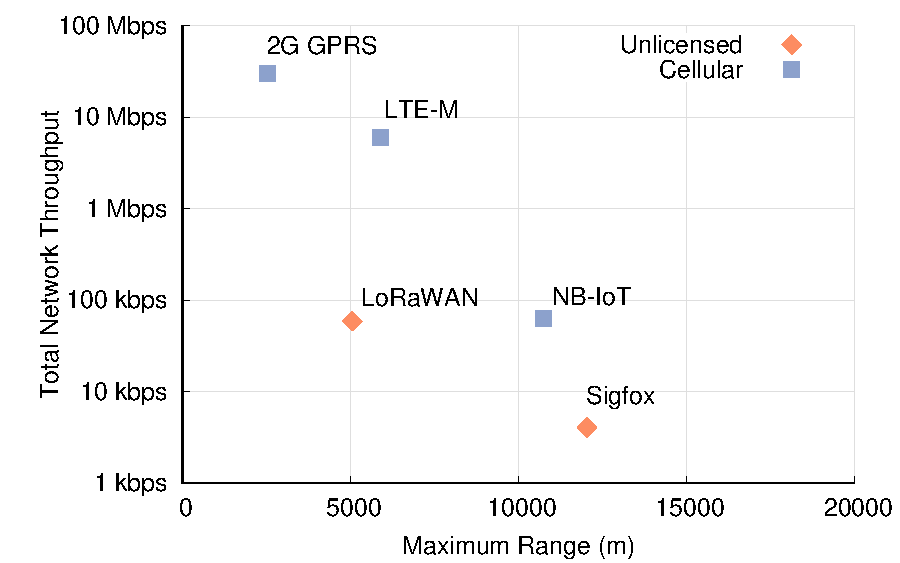
\includegraphics[width=0.49\columnwidth]{network-range-throughput}
  %\vspace{-1em}
  \caption*{\sffamily \scriptsize
   LPWANs enable low-bitrate, long-range communication.
  }
  \label{fig:lpwans}
  \vspace{-2em}
\end{wrapfigure}

\textbf{Low-Power Wide-Area Networks} (LPWANs) address a major deficit in prior
wireless networks: wide-area, machine-to-machine communications.
%
%While many solutions exist in the local-area realm,
High-power, human-centric cellular networks
%that focus on download throughput
have long been the only players if
long-range communications are desired.
%
Over the last several years, however, protocols such as LoRaWAN that operate on
the unlicensed communication bands have grown to fill this void. Their use of
simple protocols and their ability to transmit at ranges of several kilometers
while drawing only a few hundred milliwatts enables exciting new applications.

As we investigated these new networks, however, we realized that they face
significant challenges when attempting to serve real-world
applications~\cite{ghena19lpwans}.
%
%As we
%began our investigations, we realized a new metric was needed. Neither range
%nor throughput were sufficient metrics for studying LPWANs. We defined bit
%flux, a measure of throughput over coverage area as a way of comparing them.
%This metric can also be used to measure application needs which allows
%suitability to be easily measured. Comparing the bit flux requirements of
%several example applications and the bit flux that LPWANs provide, we find that
%unlicensed LPWANs are only suitable for low-rate, sparse sensing applications. 
%
LPWANs are suffering from two major issues.
%
The first is a \textit{capacity} issue: low-throughput over a very wide area
results in a very limited amount of throughput available for each deployed
device.
%
In addition to the capacity issues, LPWANs deployed in the unlicensed bands
face a \textit{coexistence} problem. The long range of these networks means
that many stakeholders will overlap in network coverage areas, especially in
urban environments.
%
These challenges are not insurmountable, but without solutions they will
ultimately stall adoption of these nascent technologies.
%These problems are not insurmountable, but neither can they be ignored. Without
%solutions, unlicensed-band, long-range networking will be eclipsed by coming
%cellular protocols.
%
%We argue that these problems must be solved in the near-term in order to allow
%unlicensed-band, long-range networking to be successful.

\textbf{Bluetooth Low Energy} (BLE) is a common communication protocol in
smartphones, laptops, and other consumer products, including many Internet of
Things devices.
%
BLE communication reduces or eliminates listening costs for energy constrained
devices, avoids interference with channel diversity, and allows
intercommunication between sensors and people through personal devices.
%
BLE advertisements---simple, periodic, broadcast messages intended for device
discovery---are used today by deployed ``beacons'' for localization and sensing
purposes.
%Using
%advertisements, a single-hop, star-topology network can be created in full
%compliance with the BLE specification that allows any number of devices to send
%data to any number of gateways[cite??].

My research has focused on understanding network models for BLE advertisements
in order to plan reliable advertisement network deployments.
%
Given the simple access control mechanisms used, many transmissions means many
packet collisions, and dense deployments could fail due to unreliable
communication.
%
%My research began by composing models that describe reception rates for BLE
%advertisements. Advertisements are sent without any coordination or
%channel-sense mechanism, essentially an ALOHA[cite] access control mechanism,
%which leads to packet collisions as a primary mechanism of data loss.
Developing analytical models for these packet collisions allows an upper bound
of reception rate for a deployed network to be determined prior to deployment
based on the number of deployed devices and their transmission rate.
%
Applying these models to results from a deployment of BLE power
meters~\cite{debruin15powerblade}, I discovered it significantly underperformed
expectations and that the gateway BLE hardware was at fault, allowing modifications
to be made for more successful future deployments.

\textbf{Future directions.}
%
%One of the biggest potential disruptors in today's low-power wireless space is
The emergence of new cellular protocols targeted at machine-to-machine
communication has a large potential for disrupting the low-power wireless
space.
%
LTE-M and NB-IoT arose from lengthy development by 3GPP and are finally
supported by network operators in the US and world-wide. Particularly these
networks could come to dominate the nascent LPWAN space, but they have
applications to the indoor space as well---the ideal of infrastructure-free
deployments is highly motivating.
%
From a resource-constrained systems view, how to successfully use these
protocols to serve application needs remains an open question.
%
While they can be low energy, they remain high power, necessitating high-latency,
batched communication to maintain energy budgets.
%Delay-tolerant network techniques may be
%helpful in order to maintain existing network primitives while dealing with
%necessary high latency.

\bigskip
\textbf{\textsf{\large Enabling Research through Platform Development.}}\\
By connecting computation and the real world, embedded systems are inhernetly
cross-disciplinary in nature.
%
Research throughout STEM fields can benefit from the creation of platforms that
can enable domain-specific research goals,
%reduce the burden of their domain-specific research goals,
and the embedded systems community has a long history of collaboration with
domain scientists.
%
I am particularly motivated by the ability to increase the impact of my research
by serving my own research interests while simultaneously providing tools for others.
%I am particularly motivated by the creation of tools that enable exploration in
%new domains that were previously burdensome to explore.

\begin{wrapfigure}{l}{0.6\columnwidth}
  \vspace{-1em}
  \centering
  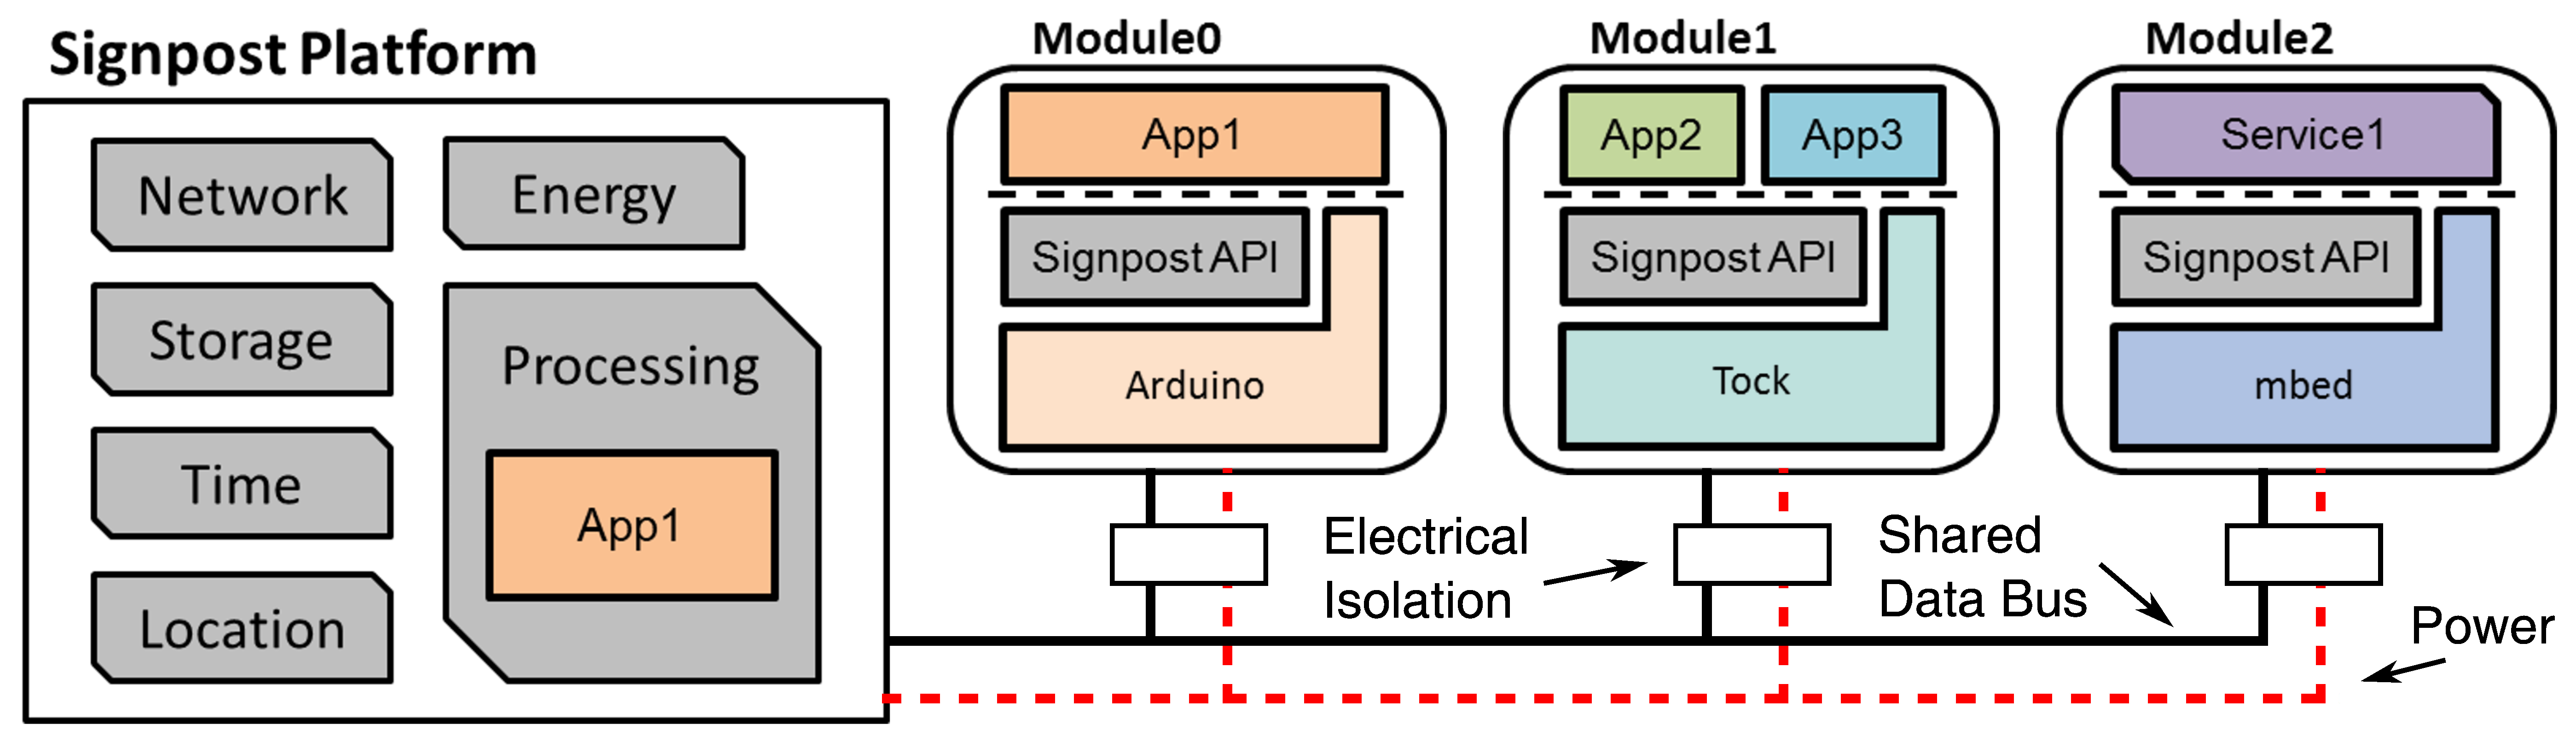
\includegraphics[width=0.59\columnwidth]{signpost_software_revised}
  %\vspace{-1em}
  \caption*{\sffamily \scriptsize
    Signpost provides shared access to services for attached application modules.
  }
  \label{fig:signpost}
  \vspace{-1em}
\end{wrapfigure}

\textbf{Signpost} aims to reduce the development burden for city-scale sensing
projects~\cite{adkins18signpost}. City-scale sensing holds a lot of
promise and interest, and for good reason: applications such as pedestrian
route planning based on air quality, noise pollution monitoring, and automatic
emergency response alerts can all improve the quality of life for a city's
inhabitants. Developing a new sensing system requires much more than just an
impactful idea, however. Hardware must be designed to support a new sensor with
energy, communications, storage, and processing capability. These requirements
make it particularly challenging to perform the short-term, exploratory research
necessary to test out ideas in the first place.

The Signpost hardware and software platform addresses these challenges by
providing commonly required resources through a modular interface. Hosted
modules provide sensors and application processing while Signpost provides
energy, network connection, storage, time, location, and
Linux-as-a-coprocessor.
%
The API for accessing these resources is abstracted
over a shared I2C bus and has been implemented for several embedded software
platforms including Tock, mbed, and Arduino.
%
Signpost supports multiple application modules simultaneously in order to
enable overlapping deployments. Resource usage is metered in order to provide
fair use across multiple tenants.
%Signpost meters shared resources such as energy and communication bandwidth in
%order to provide fairness.

\begin{wrapfigure}{}{0.5\columnwidth}
  %\vspace{-1em}
  \centering
  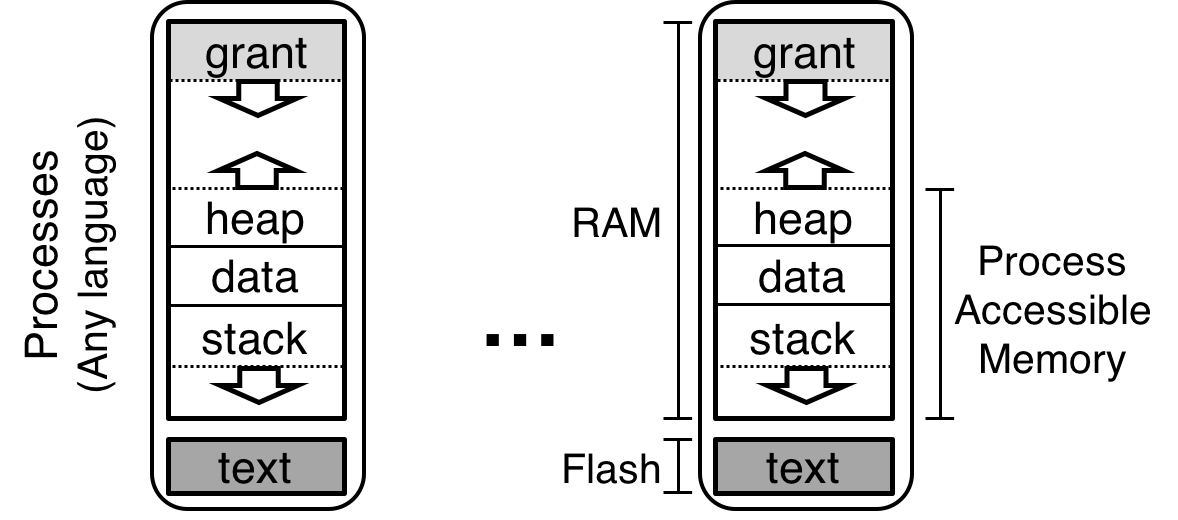
\includegraphics[width=0.49\columnwidth]{memory_layout}
  %\vspace{-1em}
  \caption*{\sffamily \scriptsize
   Tock enables multiprogramming on memory-constrained systems.
  }
  \label{fig:tock}
  \vspace{-1em}
\end{wrapfigure}

\textbf{Tock} addresses the need for modern operating systems support on
resource-constrained, microcontroller-based systems~\cite{levy17multiprogramming}.
While microcontrollers are the base compute platform for
embedded systems and the Internet of Things, OS support for them has critically
lagged behind.
Support for multiprogramming is practically nonexistent Most modern embedded
OSes compile a kernel and single application into a combined binary that is
loaded onto the microcontroller without any layered protection mechanisms.
%If you only have 64\,kB of RAM for
%the entire system sharing it was not even a consideration.

Tock demonstrates that reliable, safe, and dynamic multiprogramming is indeed
possible on memory-constrained systems. Tock enforces a system-call boundary between
applications and the kernel using new hardware features that allow for
segment-based memory protection. However, even the kernel itself is composed of
many device drivers that may not all be trustworthy. To solve this, we leverage
advancements from the programming languages community and use Rust, a type-safe
systems language with memory efficiency and performance close to C, to enforce
driver isolation~\cite{levy17rustkernel}.

\textbf{Future Directions.} Platforms research benefits not only other communities who
can use the research platform as a tool, but also my own community of embedded
systems researchers by illuminating areas that remain under-developed. While
resources like memory, processor time, and even network access are commonly
shared, energy is much less widely considered. Isolation between applications
on an energy-harvesting platform is possible but requires new policies and
APIs~\cite{adkins17energy}.

As I have developed platforms, I have recognized a trend towards
multi-microcontroller designs. Rather than handle complex software interactions
between tasks such as networking and sensing, embedded platforms have become
distributed systems, with multiple special-purpose compute modules on a single
board. While this design is increasingly common, support for it in embedded
software is entirely nonexistent, with inter-microcontroller communication
recreated in an ad hoc fashion for each platform. A need has arisen for
software primitives that support message passing, task migration, and platform
management in a principled manner for resource-constrained systems~\cite{ghena19distributed}.

%\bigskip
%\textbf{\textsf{\large Open-Source Research.}}\\
%Research,
%especially publicly funded research, should benefit the public. I am committed
%to making my research publicly available. This means not just the papers, but
%the hardware and software designs as well. Whenever possible, my first step in
%starting a new research project is creating a public Github repo for it.
%Platforms research is particularly amenable to this goal, and all hardware and
%software designs for both Signpost and Tock are publicly available.

\bigskip
\textbf{\textsf{\large Mentoring Undergraduate Research.}}\\
Working with undergraduate researchers has always been a significant part of my
research. My own experiences as an undergraduate researcher taught me both
engineering and communications skills that serve me to this day, and I want to
provide other students with that same opportunity to learn and grow. To me,
mentorship is part of the goal of academic research.
%
At Michigan, I advised nine undergraduates and two high school students working
on various projects. Five were included as authors on lab publications (mostly
demo and workshop papers, but also two conference papers) and four have gone on
to join Ph.D.\ programs in computer science, including two women.
%
I see my role as a mentor to encourage
these students to explore new domains and build deeper expertise.
%
When mentoring new students, I emphasize that they need to start with a clear
goal for what skills they're hoping to gain from their research efforts. Almost
any goals can be fit into active research projects, but the primary focus should
be ensuring that their efforts benefit them.
%%The most
%important thing is for them to have a clear goal for what skills they're hoping
%to learn in their research, then we determine how we can fit those goals to
%active research projects.
%
I am looking forward to continuing to support undergraduate research in my future
role.
%Of particular interest to me moving forward is
%supporting undergraduate teams in research and engineering efforts.


%%%%%%%%%%%%%%%%%%%%%%%%%%%%%%%%%%%%%%%%%%%%%%%%%%%%%%%%%%%%%%%%%%%%%%%%%%%%%%%%%%


\renewcommand*{\bibfont}{\footnotesize}

% https://tex.stackexchange.com/questions/22645/hiding-the-title-of-the-bibliography
\begingroup
\renewcommand{\section}[2]{}%

% title first commands
\nameusesave
\nameuse{false}

\vfill\eject
\textbf{\textsf{\Large References}}

%\bibliographystyle{plain}
%\bibliography{references}
\printbibliography

\nameuserestore

\endgroup

\end{document}

